\subsection{Tratabilidad de ASV}

Como vimos en la sección anterior, la complejidad de la distribución de entrada no es el único factor que determina la dificultad de calcular explicaciones basadas en Shapley values. De hecho, aun para distribuciones estructuralmente simples como las redes Naive Bayes, el cálculo exacto de SHAP sigue siendo intratable \cite{van2022tractability}. En contraste, los Asymmetric Shapley Values (ASV) restringen las permutaciones consideradas a aquellas compatibles con el grafo causal. En esta sección mostramos que esta restricción permite obtener tractabilidad en casos donde SHAP no la tiene.

\medskip

Consideramos el caso en que la distribución de los datos está dada por una red bayesiana Naive Bayes, y tomamos su DAG subyacente como grafo causal para calcular ASV. Recordemos que, en este caso, toda permutación topológica válida debe ubicar a la variable raíz $X_1$ antes que cualquier otra variable.

Esta observación permite caracterizar explícitamente el conjunto de órdenes topológicos y explotar la estructura de la distribución en el cálculo de ASV.

\begin{theorem}\label{the:asv_naive_bayes_tractable_clean}
	Sea $\mathcal{F}$ una familia de modelos. Los Asymmetric Shapley Values pueden calcularse en tiempo polinomial para distribuciones Naive Bayes si y solo si los Shapley values pueden calcularse en tiempo polinomial para $\mathcal{F}$ bajo distribuciones producto.
\end{theorem}

\echu{La demo es larga, la ponemos completa o damos una intuición la misma? Habría que ver el tema de si podemos mandar cosas al apéndice.}

\begin{proof}
	Primero, probamos la implicación de derecha a izquierda. Sea \(x_1\) el padre de todos los demás nodos en el DAG. Vamos a mostrar cómo calcular \(\assym_{M,e,\Pr}(x_j)\) para cualquier \(2 \leq j \leq n\) y \(\assym_{M,e,\Pr}(x_1)\) de forma independiente.
	
	Observemos que el DAG tiene \((n-1)!\) órdenes topológicos, uno para cada permutación de los features \(\{x_2, \ldots, x_n\}\), y \(\pi(x_1) = 1\) para todas ellas. Entonces,
	
	\[\label{eq:assymetric_for_naive_child}
	\assym_{M,e,\Pr}(X_j) = \sum_{\pi \in \topo(G)} w(\pi) \left[ \charactheristicFunction_{M,e,\Pr}(\pi_{<j} \cup \{x_j\}) 
	- \charactheristicFunction_{M,e,\Pr}(\pi_{<j}) \right]
	\]
	
	es equivalente a:
	
	\[
	\assym_{M,e,\Pr}(X_j) = \frac{1}{(n-1)!} \sum_{\pi \in \perm(\{x_2, \ldots, x_n\})} \left[ \charactheristicFunction_{M,e,\Pr}(\{x_1\} \cup \pi_{<j} \cup \{x_j\}) - \charactheristicFunction_{M,e,\Pr}(\{x_1\} \cup \pi_{<j}) \right]
	\]
	
	Así, una vez que \(x_1\) está fijado, la distribución para las variables \(x_2, \ldots, x_n\) es una distribución producto con \(p_{x_j} = P(X_j = 1 | X_1 = e(x_1))\). Para simplificar, asumamos que \(e(x_1) = 1\), y consideremos la distribución de producto \(\Pr'\) definida como:
	
	\[
	\Pr\,'[X_i = 1] = p_i = 
	\begin{cases}
		1 & i = 1 \\
		\Pr[X_i = 1 | X_1 = e(x_1)] & \text{en otro caso}
	\end{cases}
	\]
	
	que intuitivamente se obtiene de \(\Pr\) fijando \(X_1 = 1\). Siempre que \(x_1\) esté fijo, ambas distribuciones \(\Pr\) y \(\Pr'\) se comportan de la misma forma:
	
	
	\begin{lemma}\label{lemma:valuation_of_prob_function}
		Para cualquier \(S \subseteq X \setminus \{x_1\}\), se cumple que:
		\[
		\charFunML_{M,e,\Pr}(\{x_1\} \cup S) = \charFunML_{M,e,\Pr'}(\{x_1\} \cup S) = \charFunML_{M,e,\Pr'}(S)
		\]
	\end{lemma}
	
	\begin{proof}
		Esto se sigue de directamente manipulando la expresión:
		
		\begin{align}
			\charFunML_{M,e,\Pr}(\{x_1\} \cup S) &= \sum_{e' \in \consistsWith(e,\{x_1\} \cup S)} \Pr[e' | S] M(e') \nonumber \\
			&= \sum_{e' \in \consistsWith(e, \{x_1\} \cup S)} \left( \prod_{\substack{e'(y) = 1 \\ y \notin \{x_1\} \cup S}} p_y \prod_{\substack{e'(y) = 0 \\ y \notin \{x_1\} \cup S}} (1-p_y)\right) M(e')\\
			&= \sum_{e' \in \consistsWith(e, S)} \left( \prod_{\substack{e'(y) = 1 \\ y \notin S}} p_y \prod_{\substack{e'(y) = 0 \\ y \notin S}} (1-p_y)\right) M(e') \nonumber\\
			&= \sum_{e' \in \consistsWith(e, S)} \Pr\,'[e' | S] M(e') \nonumber\\
			&= \charFunML_{M,e,\Pr'}(S) \nonumber
		\end{align}
		
		donde la segunda igualdad viene de reemplazar $Pr$ por la distribución producto y la tercera igualdad se deduce al observar que para todas las entidades $e' \in \consistsWith(e, S)$ tales que $e'(x_1) = 0$ se cumple que 
		
		$$\prod_{\substack{e'(y) = 1 \\ y \notin S}} p_y \prod_{\substack{e'(y) = 0 \\ y \notin S}} (1-p_y) = 0$$
		
		Además, la segunda ecuación es igual a $\charFunML_{M,e,\Pr'}(\{x_1\} \cup S)$.
	\end{proof}
	
	
	%TODO: Seguir repasando esta demo y ver de entenderla bien de pi a pa
	Usando este lema, ahora demostramos
	
	\begin{align}\label{eq:relation_between_assym_and_shap_naive_child}
		\assym_{M,e,\Pr} (x_j) = \Shap_{M,e,\Pr'}(x_j)
	\end{align}
	
	Se cumple que %\sidesergio{Super menor, pero quizás en estas circunstancias siempre poner dos puntos:, o nunca}
	
	\begin{align*}
		\Shap_{M,e,\Pr'}(x_j) &= \frac{1}{n!} \sum_{\pi \in \perm(X)} \left[ \charFunML_{M,e,\Pr'}(\pi_{<j} \cup \{x_j\}) - \charFunML_{M,e,\Pr'}(\pi_{<j}) \right]\\
		&= \frac{1}{n!} \sum_{\pi \in \perm(X)} \left[ \charFunML_{M,e,\Pr'}(\{x_1\} \cup \pi_{<j} \cup \{x_j\}) - \charFunML_{M,e,\Pr'}(\{x_1\} \cup \pi_{<j}) \right]\\
		&= \frac{n}{n!} \sum_{\pi \in \perm(\{x_2,\ldots,x_n\})} \left[ \charFunML_{M,e,\Pr'}(\{x_1\} \cup \pi_{<j} \cup \{x_j\}) - \charFunML_{M,e,\Pr'}(\{x_1\} \cup \pi_{<j}) \right] \\
		&= \frac{1}{n-1!} \sum_{\pi \in \perm(\{x_2,\ldots,x_n\})} \left[ \charFunML_{M,e,\Pr}(\{x_1\} \cup \pi_{<j} \cup \{x_j\}) - \charFunML_{M,e,\Pr}(\{x_1\} \cup \pi_{<j}) \right]\\
		&= \assym_{M,e,\Pr}(x_j)
	\end{align*}
	
	donde la segunda y cuarta igualdad se siguen del Lema~\ref{lemma:valuation_of_prob_function}, la última igualdad de la Ecuación~\ref{eq:assymetric_for_naive_child} y la tercera al observar que para cada permutación de $\perm(\{x_2,\ldots,x_n\})$ podemos construir $n$ permutaciones de $\perm(X)$ insertando $x_1$ en todos los lugares posibles, y que para cada una de estas permutaciones la expresión dentro de la suma es la misma. Así, la Ecuación~\ref{eq:relation_between_assym_and_shap_naive_child} muestra que calcular $\assym_{M,e,\Pr}(x_j)$ se reduce a calcular los valores Shapley habituales para una distribución independiente particular.
	
	Ahora consideramos $\assym_{M,e,\Pr}(x_1)$. Observemos que
	
	\begin{align*}
		\assym_{M,e,\Pr}(x_1) &= \frac{1}{|\topo(G)|} \sum_{\pi \in \topo(G)} \left[ \charFunML_{M,e,\Pr}(\pi_{<1} \cup \{x_1\}) - \charFunML_{M,e,\Pr}(\pi_{<1}) \right]\\
		&= \frac{1}{|\topo(G)|}( \charFunML_{M,e,\Pr}(\{x_1\}) - \charFunML_{M,e,\Pr}(\emptyset))
	\end{align*}
	
	%\echu{¿En esta fórmula de Shap no falta el $\frac{1}{|\topo(G)|}$? Porque sino no se estaría normalizando el resultado.}
	
	ya que para todas las permutaciones el conjunto $\pi_{<1} = \emptyset$. Además, sabemos que $\charFunML_{M,e,\Pr}(\{x_1\}) = \charFunML_{M,e,\Pr'}(\emptyset)$ por el Lema~\ref{lemma:valuation_of_prob_function}, y que
	
	\begin{align*}
		\charFunML_{M,e,\Pr}(\emptyset) &= \sum_{e' \in \entities(X)} \Pr[e] M(e)\\
		&= \sum_{\substack{e' \in \entities(X) \
				\ e'(x_1) = 1}} \Pr[e' | e'(x_1) = 1] \Pr[X_1 = 1] M (e') + \sum_{\substack{e' \in \entities(X) \\ e'(x_1) = 0}} \Pr[e' | e'(x_1) = 1] \Pr[X_1 = 0] M (e')\\
		&= \Pr[X_1 = 1] \charFunML_{M,e,\Pr'}(\emptyset) + \Pr[X_1 = 0] \charFunML_{M,e,\Pr''}(\emptyset)
	\end{align*}
	
	donde la distribución $\Pr''$ es la distribución producto obtenida al fijar $X_1 = 0$ como
	
	\begin{align*}
		\Pr \, ''[X_i = 1] = \begin{cases}
			0 & i = 0\\
			Pr[X_i = 1 | X_1 = 0] & \text{de otro modo}
		\end{cases}
	\end{align*}
	
	Finalmente,
	
	\begin{align*}
		\assym_{M,e,\Pr}(x_1) = \frac{1}{|\topo(G)|}( (1 - \Pr[X_1 = 1]) \charFunML_{M,e,\Pr'}(\emptyset) - \Pr[X_1 = 0] \charFunML_{M,e,\Pr''}(\emptyset))
	\end{align*}
	
	y reducimos el problema de calcular $\assym_{M,e,\Pr}(x_1)$ al de calcular la predicción promedio del modelo $M$ para dos distribuciones independientes diferentes $\Pr'$ y $\Pr''$. Según \cite{van2022tractability}[Teorema 1], se cumple que estos promedios pueden ser calculados en tiempo polinomial si y sólo si los valores de Shapley pueden ser calculados en tiempo polinomial para una distribución de producto arbitraria.
	
	La demostración de izquierda a derecha sigue al observar que una distribución producto es un caso particular de una Distribución Naive Bayes en la cual, para cualquier valor del padre $X_1$, las distribuciones condicionales son las mismas.
	
	%\echu{ ¿Debería escribir la demo de izquierda a derecha? ¿O inecesario? No se si tiene mucho sentido, ya está muy pesada la tesis} Rta: No hace falta, con esto alcanza. 
	
\end{proof}

El Teorema~\ref{the:asv_naive_bayes_tractable_clean} muestra que, a diferencia de SHAP, ASV puede ser tratable al explotar la estructura causal. En particular, esta tratabilidad depende de poder calcular eficientemente la predicción promedio. En la experimentación nos enfocamos en árboles de decisión, donde desarrollamos algoritmos polinomiales para esta tarea.

\echu{Tiene sentido el teaser de la experimentación? O saco esa oración?}

\subsection{Clases de equivalencia y relación con los órdenes topológicos}

Recordemos la definición de ASV:
\[
\assym_{M,e,\Pr}(x_i)
=
\frac{1}{|\topo(G)|}
\sum_{\pi \in \topo(G)}
\left[
\charFunML_{M,e,\Pr}(\pi_{<i}\cup\{x_i\})-\charFunML_{M,e,\Pr}(\pi_{<i})
\right].
\]

Para simplificar la notación, en esta sección tomamos $M$, $e$ y $\Pr$ fijos, y escribimos simplemente $\charactheristicFunction$ en lugar de $\charFunML_{M,e,\Pr}$. La idea es reducir la cantidad de órdenes topológicos sobre los cuales evaluamos $\charactheristicFunction$, agrupando aquellos que devuelven el mismo resultado al evaluarse sobre $\charactheristicFunction$.

La relación ideal sería identificar dos órdenes topológicos $\pi^1,\pi^2 \in \topo(G)$ cuando
\[
\charactheristicFunction(\pi^1_{<i})=\charactheristicFunction(\pi^2_{<i}),
\]
pero esta condición es costosa de verificar, ya que requiere evaluar explícitamente la función característica. Por este motivo trabajamos con una relación más fina, puramente combinatoria.

\begin{definition}\label{def:equiv_relation_left_right}
	Sea $G=(V,E)$ un DAG y sea $x_i\in V$. Definimos la relación $\rel$ sobre $\topo(G)$ por
	\[
	\pi^1 \rel \pi^2
	\iff
	\{\pi^1_{<i}\}=\{\pi^2_{<i}\}.
	\]
	Es decir, dos órdenes topológicos son equivalentes si tienen exactamente el mismo conjunto de nodos a la izquierda de $x_i$.
\end{definition}

Esta relación depende únicamente de la posición relativa de los nodos respecto de $x_i$. Para representarla, resulta útil dividir los nodos del grafo en ancestros, descendientes y nodos no relacionados con $x_i$.

\begin{figure}[ht]
	\centering 
	\begin{tikzpicture}[scale=.95, transform shape]
		
		% ---- NODOS ----
		\node[nodo] (a1) at (0, 0) {$a_1$};
		\node[nodo] (a2) at (2.5, 2) {$a_2$};
		\node[nodo] (a3) at (2.5, -2) {$a_3$};
		\node[nodo] (xi) at (5, 0) {$x_i$};
		\node[nodo] (d_1) at (7.5, 2) {$d_1$};
		\node[nodo] (d_2) at (10, -2) {$d_2$};
		\node[nodo] (d_3) at (10, 0) {$d_3$};
		
		\node[draw=none, fill=none] (hijo_a3) at (3.5, -3) {};
		\node[draw=none, fill=none] (hijo_d2) at (9, -3) {};
		
		% ---- ARISTAS ----
		\path [->] (a1) edge[arista, mySnake]  (xi);
		\path [->] (a2) edge[arista, mySnake]  (xi);
		\path [->] (a3) edge[arista, mySnake]  (xi);
		\path [->] (xi) edge[arista, mySnake]  (d_1);
		\path [->] (xi) edge[arista, mySnake]  (d_2);
		\path [->] (xi) edge[arista, mySnake]  (d_3);
		\path [->] (a3) edge[arista, mySnake] node[above right] {} (hijo_a3);
		\path [->] (hijo_d2) edge[arista, mySnake] node[below right] {} (d_2);
		
	\end{tikzpicture}
	\caption{Al fijar un nodo $x_i$, dividimos el resto en tres grupos: ancestros ($a$), descendientes ($d$) y nodos no relacionados. Los ancestros siempre quedan a la izquierda de $x_i$, los descendientes siempre a la derecha, y solo los nodos no relacionados no tienen una posición fija respecto de $x_i$ entre distintos órdenes topológicos.}
	\label{fig:unrelatedNodesDefinition_paper}
\end{figure}

\begin{definition}\label{def:equivalence_class}
	Sea $G=(V,E)$ un DAG y $x_i\in V$. Una clase de equivalencia $\equivalenceClass$ queda determinada por una función
	\[
	f_{\pi}:V\setminus\{x_i\}\to \{\textit{left},\textit{right}\},
	\]
	donde $f_{\pi}(v)$ indica si el nodo $v$ aparece a la izquierda o a la derecha de $x_i$ en un orden topológico $\pi$. Denotamos por $L(\equivalenceClass)$ y $R(\equivalenceClass)$ a los conjuntos de nodos etiquetados con \textit{left} y \textit{right}, respectivamente.
\end{definition}

\begin{proposition}\label{prop:grouping_asv_by_eq_classes}
	Sea $eqCl(G,x_i)$ el conjunto de clases de equivalencia inducidas por $\rel$. Entonces
	\[
	\assym_{M,e,\Pr}(x_i)
	=
	\frac{1}{|\topo(G)|}
	\sum_{\equivalenceClass \in eqCl(G,x_i)}
	|\equivalenceClass|
	\left[
	\charactheristicFunction(L(\equivalenceClass)\cup\{x_i\})
	-
	\charactheristicFunction(L(\equivalenceClass))
	\right].
	\]
\end{proposition}

\begin{proof}
	Basta particionar la suma original de ASV por clases de equivalencia. Dentro de una misma clase, todos los órdenes topológicos inducen el mismo conjunto de nodos antes de $x_i$, y por lo tanto la expresión entre corchetes es constante.
\end{proof}

\echu{¿Es muy vende humo ponerle demostración? Sino lo escribo cómo un parrafo y le pongo que es la intuición.}

La ventaja de estas clases es que no requiere evaluar $\charactheristicFunction$ para decidir si dos órdenes pertenecen a la misma. La Proposición~\ref{prop:grouping_asv_by_eq_classes} muestra que, si podemos calcular eficientemente las clases de equivalencia y sus tamaños, entonces podemos computar ASV sin enumerar todos los órdenes topológicos.

\subsection{Algoritmo exacto para el cálculo de clases de equivalencia}
\label{alg:exact_algorithm_for_equivalence_classes}

Nuestro objetivo es computar $\assym_{M,e,\Pr}(x_i)$ dado un grafo causal $G$, el cual puede expresarse como una suma sobre clases de equivalencia de órdenes topológicos respecto de $x_i$. En consecuencia, el problema se reduce a calcular el conjunto $\eqClassSizes(G,x_i)$, es decir, las clases de equivalencia junto con sus tamaños.

\subsubsection{Enfoque naive}
\label{alg:naiveAlgorithmEquivalenceClass}

Un enfoque directo consiste en generar todos los órdenes topológicos de $G$ \cite{algorithmForAllTopoSorts} y luego agruparlos en clases de equivalencia según qué nodos no relacionados aparecen antes de $x_i$. A partir de esta agrupación, se obtiene un representante por clase y su tamaño.

Si bien este procedimiento es correcto, resulta computacionalmente ineficiente. En el peor caso, el número de órdenes topológicos crece factorialmente en el tamaño del grafo, es decir, $O(n!)$, lo cual vuelve impracticable este enfoque incluso para instancias moderadas. Esto motiva la necesidad de un algoritmo exacto que evite enumerar explícitamente todos los órdenes.

\subsubsection{Estructura del \textit{dtree} y estrategia general}

Proponemos un algoritmo recursivo que explota la estructura del \dtree{} inducido por el DAG alrededor del nodo $x_i$. Particionamos los nodos en tres conjuntos: ancestros $A$, descendientes $D$ y nodos no relacionados. Dentro de estos últimos, consideramos los subárboles cuyas raíces pertenecen al conjunto $UR$ (unrelated roots).

La idea central es descomponer el problema en dos etapas:
\begin{enumerate}
	\item calcular las clases de equivalencia de cada árbol no relacionado de manera independiente;
	\item combinar dichas clases con los ancestros y descendientes para obtener las clases completas.
\end{enumerate}

Cada clase de equivalencia se representa mediante una tupla
\[
(\equivalenceClassRep, leftTopos, rightTopos),
\]
donde $leftTopos$ y $rightTopos$ representan la cantidad de órdenes topológicos posibles a la izquierda y derecha de $x_i$, respectivamente. El tamaño de la clase es entonces $leftTopos \cdot rightTopos$.

La Figura~\ref{fig:ASV_forest_example} ilustra esta partición.

\begin{figure}[H]
	\centering
	\begin{tikzpicture}[scale=.65, transform shape, 
		unrelated/.style={circle, draw=red},
		ancestor/.style={circle, draw=blue},
		wiggly/.style={decorate, decoration={snake, amplitude=.2mm, segment length=2mm}}
		]
		\node[text=blue] at (-5, 0) {Ancestors};
		\node[text=teal] at (-5, -0.5) {Descendants};
		\node[text=red] at (-5, -1) {Unrelated};        
		
		\node[ancestor] (a1) at (0, 0) {$a_1$};
		\node[unrelated] (u1) at (-1, -2) {$u_1$};
		\node[ancestor] (a2) at (1, -2) {$a_2$};
		
		\drawUnrelatedTree{u2}{-1}{-4}{$u_2$}
		\node[ancestor] (a3) at (1, -4) {$a_3$};
		\node[unrelated] (u3) at (3, -4) {$u_3$};
		
		\drawUnrelatedTree{u4}{0}{-7}{$u_4$}
		\node[ancestor] (a4) at (3, -6) {$a_4$};
		
		\node[nodo] (xi) at (3, -8) {$x_i$};
		
		\drawUnrelatedTree{r1}{6}{0}{$u_5$} 
		\drawUnrelatedTree{r2}{10}{0}{$u_6$} 
		
		\node[draw=none, fill=none] (hi) at (3, -10) {};
		
		\path [->] (a1) edge (u1);
		\path [->] (a1) edge (a2);
		\path [->] (a2) edge (u2);
		\path [->] (a2) edge (a3);
		\path [->] (a2) edge (u3);
		\path [->] (a3) edge (u4);
		\path [->] (a3) edge (a4);
		\path [->] (a4) edge (xi);      
		\path [->, teal] (xi) edge[decorate, decoration={snake}] (hi);
	\end{tikzpicture}
	\caption{Partición del grafo en ancestros, descendientes y árboles no relacionados respecto de $x_i$.}
	\label{fig:ASV_forest_example}
\end{figure}

\subsubsection{Clases de equivalencia de árboles no relacionados}

Sea $UR$ el conjunto de raíces de árboles no relacionados. Para cada $ur \in UR$, calculamos recursivamente sus clases de equivalencia mediante la función $\unrEqCl$.

El caso base ocurre cuando $n$ es una hoja:
\[
\unrEqCl(n)=\{(\{n_l\},1,1),(\{n_r\},1,1)\}.
\]

Para un nodo interno, combinamos las clases de equivalencia de sus hijos y consideramos dos posibilidades: ubicar $n$ a la izquierda o a la derecha de $x_i$. Esto da lugar a la siguiente recurrencia:

\begin{align}
	\unrEqCl(n) = 
	\begin{cases} 
		\{(\{n_l\},1,1),(\{n_r\},1,1)\} & \text{si $n$ es hoja} \\[1ex]
		\bigcup_{\forall mix} \union(mix,n_{left}) \;\cup\; \union(right,n_{right}) & \text{en otro caso}
	\end{cases}
\end{align}

Existe una correspondencia biyectiva entre las clases de equivalencia de un nodo y las combinaciones de clases de sus hijos, lo cual garantiza la correctitud del esquema recursivo.

\subsubsection{Combinación con descendientes}

Los descendientes de $x_i$ siempre aparecen a la derecha, por lo que pueden tratarse como un bloque independiente. El número de órdenes topológicos de un \dtree{} enraizado en $n$ está dado por:

\begin{align}
	topoSorts(n)=
	\binom{\sum_{j} |T_{n_j}|}{|T_{n_1}|,\dots,|T_{n_{|n|}}|}
	\prod_{j} topoSorts(n_j),
\end{align}

lo cual refleja la intercalación de los órdenes de los subárboles hijos.

\subsubsection{Combinación con ancestros}

\echu{¿Debería explicar un poco menos en esta sección y meter menos fórmulas? La puedo escribir más por arriba.}

A diferencia de los descendientes, los ancestros imponen restricciones de precedencia. No es posible intercalar libremente nodos no relacionados con ancestros mediante coeficientes multinomiales.

Para resolver este problema definimos la función $leftOrders$, que contabiliza cuántas formas válidas existen de intercalar los nodos no relacionados (ubicados a la izquierda) con los ancestros, respetando las dependencias del DAG.

La Figura~\ref{fig:order_of_ancestors} ilustra una posible disposición de los ancestros.

\begin{figure}[ht]
	\centering
	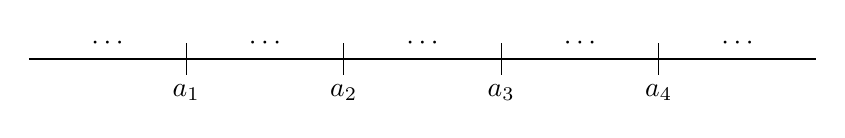
\begin{tikzpicture}
		\draw[thick] (0,0) -- (10,0);
		\foreach \x/\label in {2/$a_1$, 4/$a_2$, 6/$a_3$, 8/$a_4$} {
			\node at (\x-1,0.2) {$\cdots$};
			\draw (\x,0.2) -- (\x,-0.2);
			\node[below] at (\x,-0.2) {\label};
		};
		\node at (9,0.2) {$\cdots$};
	\end{tikzpicture}
	\caption{Orden relativo de los ancestros.}
	\label{fig:order_of_ancestors}
\end{figure}

\begin{algorithm}
	\caption{leftOrders}
	\begin{enumerate}
		\item Determinar la posición del siguiente ancestro.
		\item Elegir nodos disponibles para ubicar antes de dicha posición.
		\item Actualizar el conjunto de nodos restantes.
		\item Continuar recursivamente.
	\end{enumerate}
\end{algorithm}

\subsubsection{Fórmula final}

Integrando ambos componentes, obtenemos que el conjunto completo de clases de equivalencia puede construirse a partir del producto cartesiano de las clases de equivalencia de los árboles no relacionados. Formalmente,

\begin{align}
	\eqClassSizes(G, x_i) = 
	\bigcup_{\forall mix \in \unrEqCl(ur_1)\times\dots\times\unrEqCl(ur_{|UR|})}
	\left(eqCl(A,D,mix),\eqClassSize(A,D,mix)\right).
\end{align}

Aquí, cada $mix$ representa una elección de clases de equivalencia para cada árbol no relacionado. A partir de dicha elección, la función $eqCl(A,D,mix)$ construye la representación completa de la clase, mientras que $\eqClassSize(A,D,mix)$ calcula su tamaño combinando:

\begin{itemize}
	\item la cantidad de intercalaciones válidas con los ancestros, dada por $leftOrders$;
	\item la cantidad de órdenes topológicos de los descendientes;
	\item y las contribuciones internas de los árboles no relacionados.
\end{itemize}

De este modo, la expresión anterior no solo enumera todas las clases de equivalencia, sino que también computa exactamente su cardinalidad, sin necesidad de generar explícitamente los órdenes topológicos.

\subsubsection{Complejidad}

La complejidad total del algoritmo está dominada por dos componentes principales:

\begin{itemize}
	\item el cálculo de $\unrEqCl$, que recorre recursivamente los árboles no relacionados y combina las clases de sus hijos;
	\item la combinación global de clases, que requiere procesar el producto cartesiano de dichas clases y, para cada combinación, computar $leftOrders$ y las contribuciones de los descendientes.
\end{itemize}

En consecuencia, el costo total puede expresarse como proporcional al número de combinaciones de clases de equivalencia generadas, multiplicado por el costo de combinarlas con ancestros y descendientes. En particular, si denotamos por $k$ el número total de clases de equivalencia resultantes, el algoritmo tiene complejidad del orden de $O(k^3 \cdot \text{poly}(n))$.

Si bien $k$ puede ser exponencial en el peor caso, este enfoque evita depender del número total de órdenes topológicos del grafo, que puede ser factorial. Por lo tanto, el algoritmo representa una mejora sustancial respecto del enfoque naive, especialmente en grafos donde el número de clases de equivalencia es significativamente menor que el número de órdenes topológicos.

\subsection{Aproximación de ASV mediante sampleo}

En las secciones anteriores nos concentramos en algoritmos exactos para calcular $ASV$, ya sea enumerando todas las clases de equivalencia o explotando su estructura para reducir la cantidad de evaluaciones de la función característica. Sin embargo, cuando el número de clases o de órdenes topológicos es demasiado grande, incluso estos enfoques pueden volverse prohibitivamente costosos. Esto motiva la consideración de algoritmos aproximados basados en técnicas de muestreo.

Siguiendo la idea de las clases de equivalencia, proponemos reemplazar la suma exacta que define $ASV$ por un promedio empírico sobre una muestra aleatoria. Este enfoque permite estimar el valor de $ASV$ con buena precisión utilizando una cantidad moderada de muestras, ya que el error del estimador decrece con el tamaño de la muestra.

Existen dos variantes naturales de esta estrategia. La primera consiste en samplear órdenes topológicos del DAG causal $G$ y estimar el valor de $ASV$ a partir de sus contribuciones marginales. La segunda consiste en samplear clases de equivalencia y utilizar un representante de cada clase para aproximar el promedio exacto.

En ambos casos, el punto central es disponer de un mecanismo que permita generar muestras con la distribución correcta (uniforme en el caso de órdenes topológicos, o proporcional al tamaño en el caso de clases de equivalencia). Bajo esta condición, el cálculo de $ASV$ se reduce a promediar evaluaciones de la función característica sobre muestras i.i.d.

Una ventaja fundamental de este enfoque es que desacopla el cálculo de $ASV$ de la estructura específica del grafo. En particular, mientras que los algoritmos exactos desarrollados anteriormente explotan propiedades estructurales como la de los \dtrees{} o polytrees, el enfoque basado en sampleo puede aplicarse a \emph{cualquier} DAG, siempre que se disponga de un procedimiento para generar muestras adecuadas. Esto amplía significativamente el alcance práctico del método.

El caso de órdenes topológicos resulta especialmente natural, ya que
\[
\assym_{M,e,\Pr}(x_i)
=
\frac{1}{|\topo(G)|}
\sum_{\pi \in \topo(G)}
\left[
\charFunML_{M,e,\Pr}(\pi_{<i}\cup\{x_i\})
-
\charFunML_{M,e,\Pr}(\pi_{<i})
\right]
\]
puede interpretarse como el valor esperado de la variable aleatoria
\[
Z_\pi =
\charFunML_{M,e,\Pr}(\pi_{<i}\cup\{x_i\})
-
\charFunML_{M,e,\Pr}(\pi_{<i}),
\qquad \pi \sim \mathrm{Unif}(\topo(G)).
\]
Por lo tanto, si podemos samplear órdenes topológicos uniformemente, obtenemos un estimador insesgado de $ASV$ promediando copias i.i.d.\ de $Z_\pi$. Además al tener algoritmos de sampleo de órdenes topologicos para DAGs en general y no solo \dtrees este algoritmo logra ser más general. 

También a partir de estos órdenes sampleados podemos dividirlos por sus clases de equivalencia al igual que el algoritmo naive con probabilidad proporcional a su tamaño y estimar el valor mediante el promedio de sus representantes. Veamos a continuación dos posibles estrategias de sampleo. 

\subsubsection{Sampleo uniforme de órdenes topológicos}
\label{subsubsection:toposort_sampling}

Nos concentramos en el problema de samplear órdenes topológicos de un DAG de manera uniforme. Un primer enfoque consiste en generar todos los órdenes topológicos mediante un algoritmo determinístico, como el de Knuth \cite{algorithmForAllTopoSorts}, y devolverlos a medida que se producen. Sin embargo, este procedimiento no resulta adecuado para sampleo: al ser determinístico, no genera una distribución uniforme y puede sesgar la muestra cuando distintos nodos fuente aparecen con frecuencias muy diferentes como comienzo de un orden.

La idea correcta consiste en construir el orden de manera recursiva. Sea $S$ el conjunto de nodos fuente de un DAG $D$. Para cada $s \in S$, definimos
\[
p(s)=\frac{\#\topo(D-\{s\})}{\#\topo(D)},
\]
donde $\#\topo(D-\{s\})$ es la cantidad de órdenes topológicos que comienzan con $s$. El algoritmo selecciona el primer nodo del orden según esta distribución y luego continúa recursivamente sobre el grafo restante.

Este procedimiento garantiza que los órdenes topológicos se generan con la distribución uniforme deseada, siempre que se disponga de un método para contar la cantidad de órdenes de los subgrafos. En nuestro caso, esto se logra mediante el algoritmo de conteo desarrollado previamente para polytrees.

\echu{¿Agrego la imagen para ilustrar este algoritmo o al pedo? Me parece que no porque no le deberíamos dar mucha bola, no es tan relevante.}

Aún así, el problema que tiene este algoritmo es que solo funciona para el caso de polytrees, y sabemos que además el conteo en DAGs generales es \sharpPhard, por lo que buscamos otra estrategía de sampleo distinta.

\echu{Agregar acá lo del algoritmo de sampleo para el caso general, acá tendría que implementarlo y contar que hicimos un experimento para ver cuál era mejor para el caso de un polytree, así comparamos los tiempos. }

\subsubsection{Error del sampleo}

El esquema de aproximación basado en sampleo depende de dos subrutinas: la capacidad de generar muestras y la de evaluar la función característica sobre cada una de ellas. En particular, el algoritmo consiste en samplear independientemente órdenes topológicos y promediar sus contribuciones marginales.

Más precisamente, si $\pi^{(1)},\dots,\pi^{(m)}$ son órdenes topológicos sampleados uniformemente, el estimador viene dado por
\[
\widehat{ASV}
=
\frac{1}{m}\sum_{j=1}^{m}
\left[
\charFunML_{M,e,\Pr}(\pi^{(j)}_{<i}\cup\{x_i\})
-
\charFunML_{M,e,\Pr}(\pi^{(j)}_{<i})
\right].
\]

Cada muestra requiere generar un orden topológico y evaluar la función característica una cantidad constante de veces. La cantidad de muestras necesarias para obtener una buena aproximación depende de la precisión deseada y puede acotarse mediante resultados estándar de concentración, como se detalla en el apéndice.

\echu{¿Hay apéndice? Si no hay apéndice, meto las demostraciones que tenemos sobre la estimación del error promedio acá? } 

De manera análoga, este enfoque puede aplicarse utilizando clases de equivalencia en lugar de órdenes topológicos, siempre que se puedan samplear con la distribución adecuada.

\echu{Queda medio raro meter esta sección acá, tal vez extraería la parte de la predicción promedio en una sección más y luego metería esto al final para poner algo de la experimentación. }

\subsection{Instanciaciones particulares}
\label{section:particular_instances}

En nuestro caso, nos enfocamos en árboles de decisión como modelo $M$, y en distribuciones $\Pr$ representadas mediante redes bayesianas. En este contexto, desarrollamos un algoritmo para calcular
\[
\charFunML_{M,e,\Pr}(S)
\]
basado en recorrer el árbol de decisión y acumular las condiciones de camino inducidas por cada rama. Para cada hoja compatible con la evidencia, se computa su probabilidad mediante inferencia en la red bayesiana y se pondera por la predicción de la hoja. La predicción promedio se obtiene sumando estos aportes.

Cuando la red bayesiana tiene estructura de polytree, la inferencia puede realizarse en tiempo polinomial, por lo que el costo de evaluar la función característica es también polinomial.

Esto induce un esquema general para calcular $ASV$: siempre que el sampleo/generación exacta de órdenes topológicos o clases de equivalencia sea eficiente, se obtiene un algoritmo aproximado cuyo costo total es polinomial en el tamaño de la instancia y en los parámetros de precisión.

Por el contrario, cuando la predicción promedio no puede calcularse eficientemente, este enfoque deja de ser aplicable. En particular, el Teorema~\ref{the:asv_naive_bayes_tractable_clean} sugiere que la tratabilidad de $ASV$ está intrínsecamente ligada al costo de computar dichas esperanzas, ya que cada muestra requiere evaluar una contribución marginal.

En síntesis, los algoritmos propuestos resultan especialmente efectivos en escenarios donde:
\begin{enumerate}
	\item el sampleo/conteo puede realizarse eficientemente;
	\item la predicción promedio es computable en tiempo polinomial;
	\item el número de órdenes o clases es demasiado grande para un enfoque exacto.
\end{enumerate}

Este es precisamente el régimen considerado en la experimentación.

\echu{Acá no mostre nada de la experimentación que queríamos contar en teoría, siento que para el flow debería venir acá. ¿Que experimentos metemos? Yo banco "Clases de equivalencia vs Órdenes Topológicos" y "ASV exacto sin EqClasses vs ASV aproximado"}

\subsection{ASV exacto}

Recordemos la fórmula introducida en la sección \ref{Section:HeuristicaASV} para ASV, utilizando nuestra heurística.

\begin{align*}
	\phi_{i}^{assym}(\charactheristicFunction) = \sum_{\pi \in \perm(\players)} w(\pi) \left[ \charactheristicFunction(\pi_{<i} \cup {i}) - \charactheristicFunction(\pi_{<i}) \right] &= \\
	\heuristicASVFormula
\end{align*}

Dado un DAG $G$, un nodo $x_i \in V(G)$ y una función característica $\charactheristicFunction$. Nuestro algoritmo completo queda así entonces: 

\begin{itemize}
	\item Calculamos $eqClass$ a través de $\eqClassSizes(G,x_i)$, el algoritmo que introducimos en la sección~ \ref{alg:exact_algorithm_for_equivalence_classes}
	\item Luego para cada clase de equivalencia vamos a calcular el promedio teniendo en cuenta los features previos a $x_i$. Para realizar el promedio vamos a utilizar el algoritmo de la sección \ref{section:particular_instances}. (En el caso de que el modelo no sea un árbol, podemos aproximarlo utilizando Monte Carlo u otro método)
	\item Por último sumamos los resultados para obtener él $\assym$ para el feature $i$. 
\end{itemize}

Las modificaciones que introducimos son para mejorar la performance del mismo, sin modificar los resultados obtenidos a diferencia del enfoque aproximado. En la sección a continuación vamos a ver cuál es la mejora respecto al enfoque naive y el tiempo que tarda para distintas redes.  

\subsection{ASV aproximado}

Este algoritmo es igual al anterior. La única diferencia que tiene es respecto a cómo se calculan las clases de equivalencia, $eqClass(G, x_i)$, puesto que ahora las vamos a aproximar. Además, vamos a tener que agregar un parámetro extra, para definir la cantidad de órdenes topológicos que queremos generar. 
Primero utilizamos los algoritmos vistos en \ref{subsubsection:toposort_sampling} para samplear los órdenes topológicos. Esto nos va a permitir calcular él $ASV$ para polytrees o DAGs y no simplemente \dtrees. Luego procesamos estos órdenes al igual que en la sección \ref{alg:naiveAlgorithmEquivalenceClass}, para obtener las clases de equivalencia. Una vez obtenidas las clases de equivalencia, repetimos el mismo proceso del algoritmo exacto. 
